\documentclass[UTF8]{ctexart}

\usepackage[margin=2.4cm]{geometry}
\usepackage{amsmath, amssymb}
\usepackage{listings}
\usepackage{xcolor}
\usepackage{enumitem}
\usepackage{graphicx}
\usepackage{float}
\usepackage[colorlinks=true, linkcolor=blue, urlcolor=blue]{hyperref}

\definecolor{codebg}{HTML}{F7F7F7}
\lstset{
  basicstyle=\ttfamily\small,
  columns=fullflexible,
  keepspaces=true,
  breaklines=true,
  frame=single,
  framerule=0.3pt,
  rulecolor=\color{gray!45},
  numbers=left,
  numberstyle=\tiny\color{gray},
  xleftmargin=2.2em,
  framexleftmargin=0.6em,
  commentstyle=\color{gray!55},
  keywordstyle=\color{blue!75!black}\bfseries,
  stringstyle=\color{red!70!black},
  showstringspaces=false,
  tabsize=2,
  backgroundcolor=\color{codebg},
}

\newcommand{\cmd}[1]{\texttt{#1}}

% 插图快捷命令：#1=文件名 #2=标题
\newcommand{\shot}[2]{%
  \begin{figure}[H]\centering
    \includegraphics[width=0.72\linewidth]{figs/#1}
    \caption{#2}
  \end{figure}%
}

\title{\bfseries 系统开发工具基础 · 实验报告（第 2 周）}
\author{姓名：甘如嫣\quad 学号：25090032014}
\date{2026 年 9 月 8 日}

\begin{document}
\maketitle

\noindent\textbf{授课内容：} 命令行环境；开发环境与工具；Debugging and Profiling。

\setlist[itemize]{itemsep=2pt, topsep=3pt, leftmargin=2em}

% ===================================================================
\section{GitHub 仓库与提交记录}

本次课程的\textbf{报告、练习、代码}均已上传至个人 GitHub 仓库，采用\textbf{增量提交}（分多次 commit，禁止单次全量提交）：

\begin{center}
\url{https://github.com/ganruyan/system-basics-tools}
\end{center}

本周（第 2 周）的提交按内容拆分为 8 次独立 commit，例如：

\begin{lstlisting}[language=bash]
bc6a7a8 chore: 忽略 IDE 和 Python 缓存目录
a34cda7 week2: 第2周实验报告（LaTeX 源码 + PDF）
83bb696 week2: q05 信号与任务控制（worker.sh）
dcf669a week2: q06 语义重构
984ab11 week2: q07 归并排序调试修复
c7ce5ed week2: q08 词频程序优化
99f403f week2: 各题完整指令与课后练习 11 实例
cc06b2f fix(week2): 修正 q07 测试期望值笔误（多一个 4 致 1 failed）
\end{lstlisting}

每次提交只针对一个逻辑单元（一个题、一份报告或一项配置），保留了清晰的提交历史，便于追踪与回滚。GitHub 上的 commit 记录截图如下：

\begin{figure}[H]\centering
  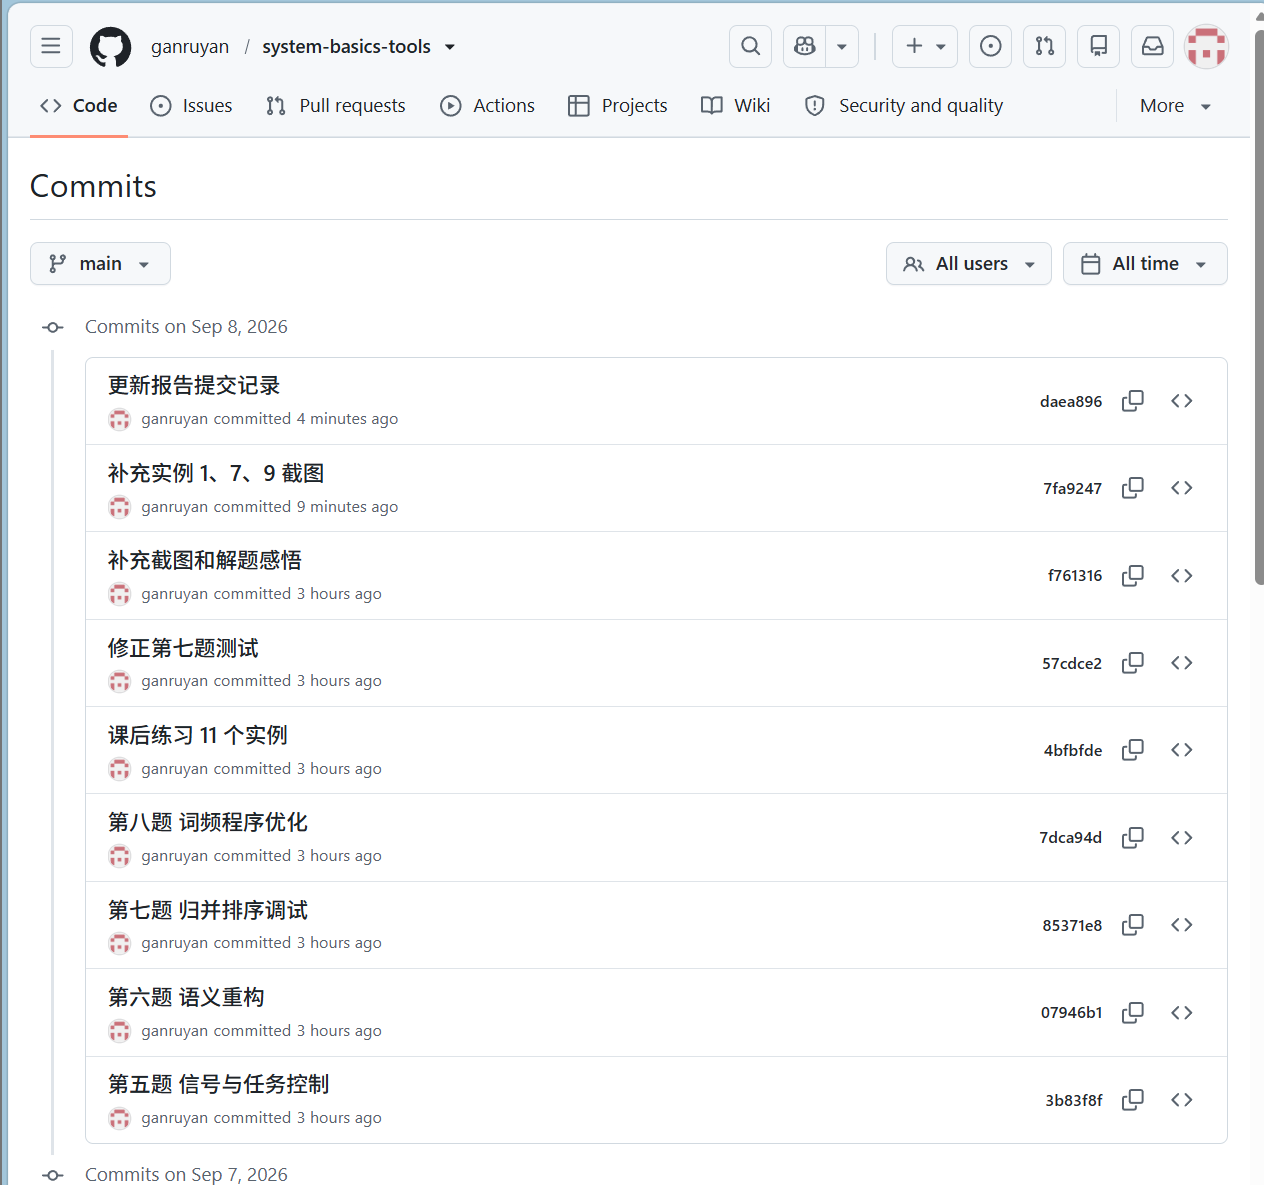
\includegraphics[width=\linewidth]{figs/commit_records.png}
  \caption{GitHub 仓库 commit 记录（\texttt{ganruyan/system-basics-tools}，\texttt{main} 分支）}
\end{figure}

% ===================================================================
\section{第 5 题\quad 控制一个可清理的后台任务}

\textbf{主题：} 命令行环境：进程、信号与任务控制 \qquad \textbf{建议用时：} 12--15 分钟

\textbf{实验目的：} 掌握前台/后台任务切换、挂起（\cmd{Ctrl-Z}）、\cmd{jobs}/\cmd{bg} 任务控制，以及用信号优雅终止可清理的任务。

\textbf{实验步骤：} 将给定脚本保存为 \cmd{q05/worker.sh} 后执行：

\begin{lstlisting}[language=bash]
cd q05
chmod +x worker.sh
./worker.sh > stdout.log 2> stderr.log    # 前台启动，stdout/stderr 分开重定向
# 按 Ctrl-Z 挂起前台任务
bg                                         # 放入后台继续运行
jobs                                       # 确认状态：[1]+ Running ...
PID=$(jobs -p)                             # 取得 PID（不手抄）
kill -TERM "$PID"                          # 发送 SIGTERM
wait "$PID" 2>/dev/null                    # 等待任务结束
cat cleanup.log                            # 应出现 CLEAN_EXIT
\end{lstlisting}

\textbf{实验结果：} \cmd{jobs} 显示任务处于 \cmd{Running} 状态；发送 \cmd{SIGTERM} 后任务退出，\cmd{cleanup.log} 中出现 \cmd{CLEAN\_EXIT}；全程未使用 \cmd{kill -9}。

\shot{q05_signal.png}{第 5 题：\cmd{worker.sh} 启动、\cmd{bg}/\cmd{jobs} 任务控制与 \cmd{CLEAN\_EXIT} 输出}

\textbf{说明：} 脚本顶部的 \cmd{trap '...' TERM INT} 捕获终止信号，先写入 \cmd{cleanup.log} 再 \cmd{exit 0}，实现优雅退出。\cmd{jobs -p} 直接返回任务 PID，避免手工抄写带来的误差。补充练习中还通过 \cmd{sleep 10000} 配合 \cmd{pgrep}/\cmd{pkill} 验证了按名称查找并终止后台任务：

\shot{q05_signal2.png}{补充：\cmd{sleep 10000} 后台任务 + \cmd{bg}/\cmd{jobs}/\cmd{pgrep}/\cmd{pkill} 控制}

% ===================================================================
\section{第 6 题\quad 语义重构与本地开发反馈}

\textbf{主题：} 开发环境与工具 \qquad \textbf{建议用时：} 12--15 分钟

\textbf{实验目的：} 使用编辑器的 Python 语言服务器完成跳转、查找引用与符号重命名，并用 \cmd{ruff} 与 \cmd{pytest} 获得本地反馈。

\textbf{实验步骤：}
\begin{enumerate}[itemsep=2pt, topsep=3pt]
  \item 在 \cmd{q06} 中按题目创建 \cmd{math\_utils.py}、\cmd{app.py}、\cmd{test\_math\_utils.py} 三个文件。
  \item 在 PyCharm 中打开 \cmd{q06}，启用 Python 语言服务器。
  \item 对 \cmd{total\_price} 分别执行\textbf{跳转到定义}（\cmd{Ctrl+B}）与\textbf{查找引用}（\cmd{Alt+F7}）。
  \item 使用\textbf{重命名符号}（\cmd{Shift+F6}）把 \cmd{total\_price} 改为 \cmd{calculate\_total}，定义与两处引用同步更新。
  \item 在 \cmd{app.py} 中临时加入未使用的 \cmd{import os}，用 \cmd{ruff} 检测并删除该行。
  \item 运行 \cmd{ruff check} 与 \cmd{pytest}，保证全部通过。
\end{enumerate}

\shot{q06_files.png}{第 6 题：\cmd{q06} 中三个文件 \cmd{math\_utils.py}/\cmd{app.py}/\cmd{test\_math\_utils.py}}

\textbf{跳转到定义与查找引用：} 光标置于 \cmd{total\_price} 上，\cmd{Ctrl+B} 跳到 \cmd{math\_utils.py} 中的定义，\cmd{Alt+F7} 列出全部引用位置。

\shot{q06_definition.png}{\cmd{total\_price} 跳转到定义 / 查找引用（语言服务器）}

\textbf{重命名符号：} \cmd{Shift+F6} 把 \cmd{total\_price} 重命名为 \cmd{calculate\_total}，三处（定义 + 两处引用）同步更新：

\begin{lstlisting}[language=Python]
# math_utils.py
def calculate_total(price: float, count: int) -> float:
    return price * count

# app.py
from math_utils import calculate_total
print(calculate_total(12.5, 4))

# test_math_utils.py
from math_utils import calculate_total
def test_total_price():
    assert calculate_total(12.5, 4) == 50.0
\end{lstlisting}

\shot{q06_rename.png}{重命名符号后 \cmd{total\_price} $\to$ \cmd{calculate\_total} 同步生效}

\textbf{实验结果：} 加入未使用的 \cmd{import os} 后，\cmd{ruff check} 报错（\cmd{F401 os imported but unused}）；删除该行后 \cmd{ruff check} 无告警；\cmd{pytest} 输出 \cmd{1 passed}。

\shot{q06_ruff.png}{\cmd{ruff check} 报出未使用的 \cmd{import os}}

\shot{q06_pytest.png}{\cmd{pytest} 输出 \cmd{1 passed in 0.01s}}

\textbf{说明：} 符号重命名是语义级重构，由语言服务器统一改写定义与所有引用，避免手工遗漏。未使用的导入由 \cmd{ruff}（基于 AST 的 linter）发现并删除，保持代码整洁。

% ===================================================================
\section{第 7 题\quad 用调试器定位归并排序缺陷}

\textbf{主题：} Debugging \qquad \textbf{建议用时：} 12--15 分钟

\textbf{实验目的：} 使用调试器定位并修复归并排序中的下标缺陷，并补充测试保证正确性。

\textbf{实验步骤：}
\begin{enumerate}[itemsep=2pt, topsep=3pt]
  \item 将缺陷代码保存为 \cmd{q07/merge\_sort.py} 并运行，输出 \cmd{[1, 5, 4, 3, 4, 5, 6, 9]}，与正确的 \cmd{[1, 1, 2, 3, 4, 5, 6, 9]} 不符。
  \item 在 \cmd{merge} 函数设断点，单步观察 \cmd{i}、\cmd{j}、\cmd{left}、\cmd{right} 的取值变化。
  \item 定位缺陷：\cmd{else} 分支误用 \cmd{right[i]}，应为 \cmd{right[j]}。
  \item 完成最小修复（不替换为 \cmd{sorted}）。
\end{enumerate}

\shot{q07_bug.png}{第 7 题：缺陷代码输出乱序结果 \cmd{[1, 5, 4, 3, 4, 5, 6, 9]}}

\shot{q07_debug.png}{调试器断点观察变量：\cmd{else} 分支应取右侧指针 \cmd{j} 对应的元素}

\textbf{缺陷位置与修复：}

\begin{lstlisting}[language=Python]
while i < len(left) and j < len(right):
    if left[i] <= right[j]:
        result.append(left[i]); i += 1
    else:
        result.append(right[j]); j += 1   # 原为 right[i]，已修复
\end{lstlisting}

\shot{q07_fixed.png}{修复后输出正确结果 \cmd{[1, 1, 2, 3, 4, 5, 6, 9]}}

\textbf{补充测试：}

\begin{lstlisting}[language=Python]
# test_merge_sort.py
from merge_sort import merge_sort

def test_given_input():
    assert merge_sort([3, 1, 4, 1, 5, 9, 2, 6]) == [1, 1, 2, 3, 4, 5, 6, 9]

def test_duplicates():
    assert merge_sort([5, 3, 5, 1, 3, 1]) == [1, 1, 3, 3, 5, 5]
\end{lstlisting}

\shot{q07_pytest.png}{\cmd{pytest} 运行两个测试（图为首轮：\cmd{test\_given\_input} 因期望值笔误失败，修正后为 \cmd{2 passed}）}

\textbf{实验结果：} 修复后运行输出正确；\cmd{pytest} 输出 \cmd{2 passed}；未使用 \cmd{sorted} 替换归并排序。

\textbf{说明：} \cmd{else} 分支对应``取右侧较小元素''，其下标应为右侧指针 \cmd{j}；误用 \cmd{i} 既可能越界，也会产生错误结果。调试时借助断点与变量面板，定位到\textbf{错误发生的确切一行}，比反复 \cmd{print} 更高效。

% ===================================================================
\section{第 8 题\quad 先测量，再优化慢速词频程序}

\textbf{主题：} Profiling \qquad \textbf{建议用时：} 12--15 分钟

\textbf{实验目的：} 用计时与 \cmd{cProfile} 先测量、定位瓶颈，再对故意低效的去重程序做优化，并量化加速效果。

\textbf{实验步骤：}

\begin{lstlisting}[language=bash]
cd q08
python generate_words.py                         # 生成 words.txt（可重复）
Measure-Command { python wordfreq.py }           # Windows 下用 Measure-Command 计时（等价 time）
Measure-Command { python wordfreq.py }           # 运行 2 次取中位数
python -m cProfile -s cumulative wordfreq.py     # 定位耗时函数/行
\end{lstlisting}

\shot{q08_generate.png}{第 8 题：\cmd{generate\_words.py} 生成 \cmd{words.txt}}

原始（低效）程序用列表判重，\cmd{count} 输出为 $1000$：

\begin{lstlisting}[language=Python]
words = open("words.txt", encoding="utf-8").read().split()
unique = []
for word in words:
    if word not in unique:     # 列表线性查找，O(n)
        unique.append(word)
print("count=", len(unique))
\end{lstlisting}

\shot{q08_count.png}{原始程序输出 \cmd{count= 1000}}

\textbf{定位结果：} \cmd{cProfile -s cumulative} 输出显示，主要耗时集中在 \cmd{if word not in unique}——在列表 \cmd{unique} 上做线性查找（\cmd{list.append} 与成员判断），整体复杂度为 $O(n^2)$。

\shot{q08_cprofile.png}{\cmd{cProfile -s cumulative} 输出：\cmd{list.append} 与成员判断是热点}

\textbf{优化（用集合做 $O(1)$ 判重）：}

\begin{lstlisting}[language=Python]
words = open("words.txt", encoding="utf-8").read().split()
unique = set()
for word in words:
    if word not in unique:     # 哈希查找，O(1)
        unique.add(word)
print("count=", len(unique))
\end{lstlisting}

\shot{q08_optimized.png}{优化后代码（\cmd{list} $\to$ \cmd{set}），\cmd{count} 仍为 $1000$}

\shot{q08_timing.png}{优化后用 \cmd{Measure-Command} 计时两次（取中位数算加速比）}

\textbf{实验结果：} 优化前后 \cmd{count} 均为 $1000$（未写死）；优化后单次耗时约 $0.05$ 秒。用相同输入再运行 2 次，分别取耗时\textbf{中位数}，计算加速比（优化前中位数 $\div$ 优化后中位数）。由于 \cmd{set} 的成员判断是 $O(1)$，整体从 $O(n^2)$ 降到 $O(n)$，输入规模越大、加速越明显。

\textbf{说明：} \cmd{cProfile -s cumulative} 按累计耗时排序，直接暴露热点。优化以集合替换列表去重，保持最终 \cmd{count} 不变，符合``先测量、再优化''的方法。

% ===================================================================
\section{课后练习：十一个实例}

本次课后练习共完成 $11$ 个实例（$>10$），覆盖参数与 Globs、IDE/语言服务器、LLM 辅助调试、进程与端口、基准测试与系统监控等主题。

\subsection{实例 1\quad ls 组合选项（参数与 Globs）}

\textbf{环境：} Windows Git Bash / Ubuntu 虚拟机。一条命令同时满足``含所有文件、易读大小、按时间排序、带颜色''：

\begin{lstlisting}[language=bash]
ls -laht --color=auto
\end{lstlisting}

各选项含义：\cmd{-l} 长格式（权限/大小/时间/名字）、\cmd{-a} 包含隐藏文件、\cmd{-h} 大小易读（\cmd{1.1M}、\cmd{106M} 而非纯字节）、\cmd{-t} 按最近修改时间排序、\cmd{--color=auto} 带颜色输出。

\textbf{结果：} 一次输出即可同时看到所有文件（含隐藏）、易读的大小、按时间倒序排列并着色。

\shot{inst01_ls.png}{实例 1：\cmd{ls -laht --color=auto} 一次输出展示隐藏文件、易读大小、按时间倒序}

\subsection{实例 2\quad 语言服务器：对库依赖跳转到定义}

\textbf{环境：} Windows · PyCharm。在代码中引用标准库函数，用 \cmd{Ctrl+B} 跳到库的定义：

\begin{lstlisting}[language=Python]
import random
print(random.choice([1, 2, 3]))
\end{lstlisting}

光标置于 \cmd{choice} 上按 \cmd{Ctrl+B}，跳到标准库 \cmd{random.py} 中的 \cmd{def choice}。

\shot{inst02_jump.png}{实例 2：跳转到标准库 \cmd{random.py} 的 \cmd{def choice} 定义}

\textbf{结果：} 成功跳转到标准库定义，验证了语言服务器对\textbf{库依赖}的跳转能力（与第 6 题跳转自己写的函数相对照）。

\subsection{实例 3\quad 安装一个 IDE 扩展}

\textbf{环境：} Windows · VS Code。在扩展面板搜索 \cmd{GitLens}（Git 增强插件，与课程 git 主题契合）并安装。

\shot{inst03_ext_search.png}{实例 3：VS Code 扩展面板搜索 GitLens}

\shot{inst03_ext_installed.png}{实例 3：GitLens 安装完成（扩展详情页）}

\textbf{结果：} GitLens 安装成功，可用于查看代码历史、Git blame 与提交图。

\subsection{实例 4\quad 用 LLM 调试晦涩报错}

\textbf{环境：} 任意（有浏览器即可）。把一段难以读懂的 C++ 模板报错粘给 LLM：

\begin{lstlisting}
error: no match for 'operator<<' (operand types are 'std::ostream'
       {aka 'std::basic_ostream<char>'} and 'std::vector<int>')
\end{lstlisting}

\shot{inst04_llm.png}{实例 4：将 C++ 模板报错交给 LLM，得到解释与修复建议}

\textbf{结果：} LLM 解释了报错原因（\cmd{std::vector} 未重载 \cmd{operator<<}），并给出三种修复方式：用 \cmd{for} 循环逐个输出、用 \cmd{std::copy} + \cmd{ostream\_iterator}、或自行重载 \cmd{operator<<}。

\subsection{实例 5\quad 排查端口被占用并结束进程}

\textbf{环境：} Windows。开两个终端，一个启动最小 Web 服务器占用 \cmd{4444} 端口，另一个排查并结束它：

\begin{lstlisting}[language=bash]
# 终端 A：占用 4444 端口
python -m http.server 4444
# 终端 B：查占用端口的进程
netstat -ano | findstr 4444      # 找到 PID（如 5916）
taskkill /PID 5916 /F            # 强制结束
\end{lstlisting}

\shot{inst05_port.png}{实例 5：\cmd{http.server 4444} 启动 + \cmd{netstat} 查到 PID 5916}

\shot{inst05_taskkill.png}{实例 5：\cmd{taskkill /PID 5916 /F} 结束占用进程}

\textbf{结果：} 通过 \cmd{netstat -ano} 定位到占用 \cmd{4444} 端口的进程 PID，\cmd{taskkill} 成功结束，终端 A 的服务随即停止。

\subsection{实例 6\quad 启用 Vim 模式}

\textbf{环境：} Windows · PyCharm。在插件中启用 \cmd{IdeaVim}，在编辑器中获得 Vim 的模态编辑体验。

\shot{inst06_vim.png}{实例 6：PyCharm 插件市场中的 IdeaVim}

\shot{inst06_vim_enabled.png}{实例 6：IdeaVim 启用后进入 \cmd{-- NORMAL --} 模式}

\textbf{结果：} 重启后编辑器右下角显示 \cmd{-- NORMAL --}，可用 \cmd{h}/\cmd{j}/\cmd{k}/\cmd{l} 移动光标、\cmd{i} 进入编辑模式。

\subsection{实例 7\quad \texttt{touch -- -myfile}，再用 \texttt{./} 前缀删除它}

\textbf{环境：} Windows Git Bash / Ubuntu 虚拟机。文件名以 \cmd{-} 开头时，用 \cmd{--} 告诉命令``后面是文件名而非选项''：

\begin{lstlisting}[language=bash]
touch -- -myfile     # -- 表示 -myfile 是文件名，不是选项
ls -la               # 能看到 -myfile
rm ./-myfile         # 用 ./ 前缀删除以 - 开头的文件
\end{lstlisting}

\textbf{结果：} \cmd{--} 让 \cmd{touch} 把 \cmd{-myfile} 当作普通文件名创建；删除时以 \cmd{./-myfile} 形式避免被解析为选项。

\shot{inst07_touch.png}{实例 7：\cmd{touch -- -myfile} 创建、\cmd{ls -la} 查看、\cmd{rm ./-myfile} 删除}

\subsection{实例 8\quad 用 strace 跟踪系统调用}

\textbf{环境：} Ubuntu 虚拟机。

\begin{lstlisting}[language=bash]
sudo apt install -y strace
strace ls -l
\end{lstlisting}

\shot{inst08_strace.png}{实例 8：\cmd{strace ls -l} 输出的系统调用（\cmd{execve}/\cmd{openat}/\cmd{mmap}/\cmd{close} 等）}

\textbf{结果：} 观察到 \cmd{ls -l} 背后的系统调用序列：\cmd{execve} 启动、\cmd{openat}/\cmd{mmap} 加载动态库、\cmd{getdents64} 读目录、\cmd{write} 输出等，直观理解程序与内核的交互。

\subsection{实例 9\quad 进程替换：用 diff 比较 printenv 与 export}

\textbf{环境：} Windows Git Bash / Ubuntu 虚拟机。用进程替换 \cmd{<(cmd)} 把命令输出当作``临时文件''传给 \cmd{diff}：

\begin{lstlisting}[language=bash]
diff <(printenv | sort) <(export | sort)
\end{lstlisting}

\textbf{结果：} 两个命令输出格式不同——\cmd{printenv} 输出 \cmd{NAME=value}，而 \cmd{export} 输出 \cmd{declare -x NAME="value"}，因此 \cmd{diff} 显示大量差异；但变量集合本质相同，只是格式不同。

\shot{inst09_procsub.png}{实例 9：进程替换 \cmd{diff <(printenv | sort) <(export | sort)} 显示两者格式差异}

\subsection{实例 10\quad 用 hyperfine 基准对比两个实现}

\textbf{环境：} Ubuntu 虚拟机。用 \cmd{hyperfine} 对比 \cmd{find} 与 \cmd{fd}（\cmd{fdfind}）：

\begin{lstlisting}[language=bash]
sudo apt install -y hyperfine ripgrep fd-find
cd ~
hyperfine 'find . -type f' 'fdfind --type f'
\end{lstlisting}

\shot{inst10_hyperfine.png}{实例 10：\cmd{hyperfine} 对比 \cmd{find} 与 \cmd{fdfind}（后者快约 5.7 倍）}

\textbf{结果：} \cmd{fdfind} 平均耗时远小于 \cmd{find}，结果报告显示约 \cmd{5.7} 倍加速，并给出均值、范围等统计信息。

\subsection{实例 11\quad 用 htop 监控系统}

\textbf{环境：} Ubuntu 虚拟机。用一个 Python 死循环占满一个 CPU 核，再用 \cmd{htop} 观察：

\begin{lstlisting}[language=bash]
sudo apt install -y htop
python3 -c "while True: pass"   # 终端 1：占满 CPU
htop                            # 终端 2：观察（q 退出）
\end{lstlisting}

\shot{inst11_htop.png}{实例 11：\cmd{htop} 显示 CPU 高占用与进程列表}

\textbf{结果：} \cmd{htop} 中可见 \cmd{python3} 进程 CPU 接近 $100\%$，实时展示负载、内存与各进程状态，按 \cmd{q} 退出。

% ===================================================================
\section{解题感悟}

（以下为初稿，已按本次实验实际内容撰写，可在提交前补充个人体会。）

\textbf{1. Git 增量提交，让历史成为可追溯的``时间线''。} 最初我会把整周内容一次性提交，历史记录毫无信息量。本次按``一个题一次提交''拆分后，每次 commit 都对应一个明确意图，回看时能立刻定位``某道题在哪次提交做了什么改动''。尤其是修复 q07 测试期望值笔误时，一条 \cmd{fix} 提交就把``发现问题 $\to$ 修正''的过程记录了下来，这正是版本控制的价值。

\textbf{2. 调试器比 \cmd{print} 更精准。} 第 7 题若只靠 \cmd{print} 会反复猜测；用调试器设断点、单步观察 \cmd{i}/\cmd{j} 两个指针，一步就锁定了 \cmd{right[i]} 应改为 \cmd{right[j]} 的缺陷。这让我体会到``定位到出错的那一行''比``打印看结果''高效得多。

\textbf{3. 先测量，再优化。} 第 8 题先用 \cmd{cProfile -s cumulative} 定位到 \cmd{list} 线性查找是热点，再决定把判重容器换成 \cmd{set}，整体从 $O(n^2)$ 降到 $O(n)$，且 \cmd{count} 结果保持不变。没有测量就去``优化''，往往是凭感觉改错了地方。

\textbf{4. 自动化测试是回归的保险丝。} 第 6、7 题用 \cmd{pytest} 写断言后，任何改动都能立刻得到反馈。测试暴露出的``期望值多写一个 4''这类笔误，也提醒我：测试本身也需要被仔细检查。

\textbf{5. 命令行工具极大提升排查效率。} \cmd{netstat} + \cmd{taskkill} 定位端口、\cmd{strace} 观察系统调用、\cmd{hyperfine} 做基准、\cmd{htop} 看负载——这些工具组合起来，能快速回答``谁占了我的端口''``程序卡在哪''``哪个实现更快''等实际问题。

\end{document}
